\section{Project Summary}

The proposed sculpture aims to embody the particle-wave duality phenomena and the quantum state collapse under observation.
By providing a large-scale physical manifestation of some core concepts in quantum theory, I hope to spark the sense of wonder quantum theory can provide in the visitors to YQI.

\begin{figure}[t]
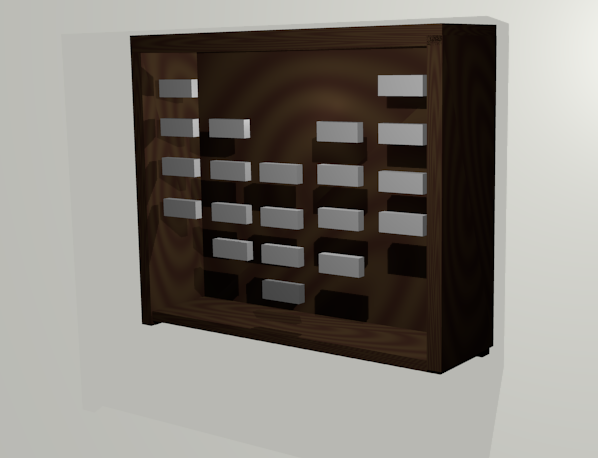
\includegraphics[width=0.48\textwidth]{../Test.png}
\label{fig:render}
\caption{A very rough render of the proposed physical installation. The top of frame will also include wooden housing for the electronics and motors (not shown).}
\end{figure}

The sculpture is a grid of metal plates installed on the wall within a wooden display case, as rendered in Fig.~\ref{fig:render}.
Each plate is controlled by a motor, giving it one degree of freedom of motion vertically.
The default motion for the plates is a wave-like pattern, as demonstrated in the demo video available at \url{https://youtu.be/mmsq-_oRCoQ}.
This video was shot in the space to test the aesthetics of various form factors.
While the exact dimensions of the sculpture are still to be determined, based on the demo video I expect roughly 60'' x 35'' x 10''.

A motion sensor is installed at the bottom of the case.
When the motion sensor is tripped (by an observer approaching the installation or sitting in the chairs), the plates switch behaviors to collectively move to, and wait at, either the top or bottom of the grid nondeterministically.
After X minutes, the plates resume their wave-like pattern. 
The motion sensor is then disabled for Y minutes\footnote{The value for X and Y remain to be experimentally determined during beta testing of installation.}.


At the moment the entire code base has been written by hand. 
As an example, we list code in Fig.~\ref{fig:code} which describes the transitions between quantum states.
While relatively intuitive, the relationship between these states and the plates' position over time is much more complicated (full code available at~\cite{github}).
Development of the code was time consuming and error-prone, so we would prefer to synthesize the code from logical specifications.
In our research group's current project we built a program which can automatically generate time-varying, interactive programs from such specifications~\cite{pldi}.
The opportunity to test this tool in a real-world, artistic setting would be an interesting challenge.
This application would also be well suited as a demo submission to the FARM workshop in the Spring of 2017.

\begin{figure}
\begin{lstlisting}
changeQState (observed,q,plates) = if
  | observed && q==Quantum -> Classic
  | observed && q==ReQuantize -> Classic
  | q==ReQuantize -> 
      if inOrigPos plates 
      then Quantum else ReQuantize
  | otherwise -> q
\end{lstlisting}
\label{fig:code}
\caption{Code as art}
\end{figure}


If accepted, and with the approval of the board, I would like to dedicate this installation to my late advisor here at Yale, Paul Hudak.
As the inventor of both FRP and a founder of Haskell, using an FRP Haskell library in a public work of art at YQI seems to capture a small part of the vision Paul had for the boundless possibilities at the intersection of logic and imagination.

\subsection{Schedule}

The following deadlines are a proposed schedule for the installation, subject to change depending on the start date.
The control code of the FRP program can be swapped out at any time, so there is no constraint from the synthesis research.
If the synthesis research is not ready for deployment when the physical structure is completed, it can also be swapping in later.

\begin{enumerate}
\item Manufacture one test set of plates on wires (Dec 10)
\item Build winding mechanism with motor (Dec 20)
\item Test build one column with manually controlled motors (Jan 3)
\item Arduino\ldots
  \begin{enumerate}
     \item controlling single motor connected to plate (Jan 12)
     \item controlling standalone motors for one column (Jan 16)
     \item controlling 20 standalone motors (Jan 20)
     \item controlling 20 motors connected to plates (Feb 1)
     \item taking input from motion sensor (Feb 10)
  \end{enumerate}
\item Begin installation in space (Feb 17)
\item Finish installation (Feb 28)
\end{enumerate}

\subsection{Budget and Materials}

Because the work for this project will be funded under my advisor's current NSF grant CCF-0811665 (which was previously Hudak's grant), I cannot accept separate payment for artist time.
I will only request funding for materials.
The below are meant to be overestimates.

\begin{table}[h!]
\centering
\caption{Itemized Budget for materials}
\label{table:results}
\vspace{0.4em}
\begin{tabular}{|l|r|r|r|}
\hline
\multicolumn{1}{|c|}{\multirow{2}{*}{\textsc{Item}}} 
  & \multicolumn{1}{c|}{\multirow{2}{*}{\scriptsize{(\$)} \textsc{/ Unit}}}
  & \multicolumn{1}{c|}{\multirow{2}{*}{\scriptsize{Quant}}}
  & \multicolumn{1}{c|}{\multirow{2}{*}{\scriptsize{Total} \scriptsize{(\$)}}} \\ 
& \multicolumn{1}{c|}{\textsc{}} & \multicolumn{1}{c|}{\textsc{}} & \\
\hline \hline
\textbf{Grid} & & & \\[-0.2em]
\quad Plates & 15 & 20 & 300  \\
\quad 5lb Fishing Line & 10 & 40ft & 10  \\
\quad Reels for line & 5 & 20 & 100  \\
\hline 
\textbf{Frame} & & & \\[-0.2em]
\quad Museum Glass & - & - & 300  \\
\quad Timber & - & - & 60  \\
\hline 
\textbf{Electronics} & & & \\[-0.2em]
\quad Arduino  & - & - & 45  \\
\quad Motion sensor & - & - & 10  \\ 
\quad NEMA17 Stepper Motor & 13 & 20 & 260  \\
\hline 
\hline 
\textbf{Total} & - & - & 1085 \\
\hline 
\end{tabular}
\end{table}

This project also require power for the motors and the Arduino. 
I plan to use the outlet to the bottom left of the space in the hallway with an extension cord.
The power-in cord for the sculpture will exit the bottom left of the frame, minimizing visual impact.

\subsection{Extensions}

This project also has the potential to be extended to capture the idea of quantum entanglement.
I hope to eventually install this same sculpture at Yale NUS in Singapore, with a small addition.
The Yale New Haven sculpture will be connected to the Yale NUS sculpture over the internet.
Whenever the motion sensor is triggered for one sculpture and collapses the state to a 0 or 1, the paired sculpture will also collapse to the complement state.


